\documentclass[12pt]{article}
\usepackage{newtxtext}
\usepackage[T1]{fontenc}
\usepackage{etoolbox}
\usepackage{booktabs}


\makeatletter
%\patchcmd{<cmd>}{<search>}{<replace>}{<success>}{<failure>}
\patchcmd{\@makechapterhead}{\huge}{\large}{}{}% for \chapter
\patchcmd{\@makechapterhead}{\Huge}{\large}{}{}% for \chapter
\patchcmd{\@makeschapterhead}{\Huge}{\large}{}{}% for \chapter*
\patchcmd{\@makeschapterhead}{\HUGE}{\large}{}{}
\makeatother

\usepackage[top=0.75in, bottom=0.75in, left= 0.75in, right=0.75in]{geometry}
\usepackage{amsmath}
\usepackage{enumitem}
\usepackage[english]{babel}
\usepackage{hyperref}
\usepackage[utf8]{inputenc}
% \usepackage{xcolor}
\usepackage[autostyle]{csquotes}
\usepackage{graphicx}
\usepackage[stable]{footmisc}
\usepackage{subfig}
\usepackage{listings}
\usepackage{floatrow}
\usepackage{textcomp}
\usepackage{multirow}
\usepackage{tabulary}
\newcolumntype{K}[1]{>{\centering\arraybackslash}p{#1}}
\usepackage[table]{xcolor}
\newfloatcommand{capbtabbox}{table}[][\FBwidth]
\usepackage{framed}

\definecolor{codegreen}{rgb}{0,0.6,0}
\definecolor{codegray}{rgb}{0.5,0.5,0.5}
\definecolor{codepurple}{rgb}{0.58,0,0.82}
\definecolor{backcolour}{rgb}{0.95,0.95,0.92}

\lstdefinestyle{mystyle}{
    backgroundcolor=\color{backcolour},   
    commentstyle=\color{codegreen},
    keywordstyle=\color{magenta},
    numberstyle=\tiny\color{codegray},
    stringstyle=\color{codepurple},
    basicstyle=\ttfamily\footnotesize,
    breakatwhitespace=false,         
    breaklines=true,                 
    captionpos=b,                    
    keepspaces=true,                 
    numbers=left,                    
    numbersep=5pt,                  
    showspaces=false,                
    showstringspaces=false,
    showtabs=false,                  
    tabsize=2
}
\lstset{style=mystyle}
\setlength{\parindent}{4em}
\setlength{\parskip}{1em}
\setcounter{tocdepth}{3} % Show sections

\usepackage[nottoc]{tocbibind}

\usepackage{pgf}
\usepackage{pgfpages}

\usepackage[style=authoryear,sorting=none]{biblatex}
\addbibresource{references.bib}

\pgfpagesdeclarelayout{boxed}
{
  \edef\pgfpageoptionborder{2pt}
}
{
  \pgfpagesphysicalpageoptions
  {%
    logical pages=1,%
  }
  \pgfpageslogicalpageoptions{1}
  {
    border code=\pgfsetlinewidth{2pt}\pgfstroke,%
    border shrink=\pgfpageoptionborder,%
    resized width=.95\pgfphysicalwidth,%
    resized height=.95\pgfphysicalheight,%
    center=\pgfpoint{.5\pgfphysicalwidth}{.5\pgfphysicalheight}%
  }%
}

\pgfpagesuselayout{boxed}


\begin{document}
%Hello
\begin{titlepage}
\begin{center}
\normalsize{A dissertation report on} \\ 
\vspace{1em}
\Large{\textbf{\enquote{Interactive Learning Platform for Orbital Mechanics Using Python}}}\\ \vspace{1em}
\normalsize{Submitted to}\\ \vspace{1em}

\includegraphics[scale=0.75]{images/AU.png}\\ \vspace{1em}
\normalsize{In partial fulfilment of the requirements for the award of degree} \\ \vspace{0.75em}
\Large{\textbf{Bachelor of Technology}}\\
\Large{\textbf{In}}\\
\Large{\textbf{Aerospace Engineering}}\\ \vspace{1em}
\normalsize \textbf{Submitted by:} \vspace*{1em} \\
\normalsize
\begin{tabular}{cc}
\textbf{Ramkiran L.} & \textbf{Manjunath} \\ 
17030141AE007 & 17030141AE009 \\ 
lramkiranBTECH17@ced.alliance.edu.in & manjunathBTECH17@ced.alliance.edu.in \vspace{1em} \\ 
\textbf{Monisha Patel A.} & \textbf{Thoshitha R. Kumar} \\ 
17030141AE013 & 17030141AE027 \\ 
pamonishaBTECH17@ced.alliance.edu.in & kuthoshithaBTECH17@ced.alliance.edu.in \vspace{0.75em} \\ 
\end{tabular} 
\normalsize

\textbf{Under the guidance of}\\
\begin{tabular}{cc}
\textbf{Prof. Gisa G.S.} & \textbf{Prof. Yadu Krishnan} \\
Assistant Professor & Assistant Professor \\
Department of Aerospace Engineering,& Department of Aerospace Engineering,\\
Alliance College of Engineering and Design, & Alliance College of Engineering and Design,\\
Alliance University, Bengaluru. & Alliance University, Bengaluru. \vspace*{1em}\\
\end{tabular}
\textbf{Department of Aerospace Engineering}\\
\textbf{Alliance College of Engineering and Design}\\
\textbf{Alliance University, Bengaluru - 562106} \\
\textbf{Batch - 2017-21}\\
\textbf{Year - 2021}
\end{center}
\end{titlepage}
\begin{center}

\includegraphics[scale=0.7]{images/AUText.png} \vspace*{2em}\\
\textbf{CERTIFICATE}
\end{center}
This is to certify that \textbf{Mr. Ramkiran L. (17030141AE007), Mr. Manjunath (17030141AE009), Ms. Monisha Patel A. (17030141AE012)} and \textbf{Ms. Thoshitha R. Kumar (17030141AE027)} students of \textbf{Aerospace Engineering, Bachelor of Technology 2017-21} batch at \textbf{Alliance College of Engineering and Design (ACED), Alliance University, Bengaluru} has completed the project report titled \textit{\textbf{\enquote{Interactive Learning Platform for Orbital Mechanics Using Python}}} under our guidance in partial fulfillment for the award of Bachelor of Technology degree in Aerospace Engineering, Alliance University, Bangalore during the year 2020-2021. \vspace{1em}\\
\begin{center}
\begin{tabular}{K{7cm} K{0.5cm} K{7cm}}
\underline{\hspace{2.9cm}} & & \underline{\hspace{4.3cm}} \\ 
\textbf{Prof. Gisa G.S} & & \textbf{Prof. Yadu Krishnan} \vspace{1em}\\ 
Internal Guide & &  Internal Guide\\ 
Department of Aerospace Engineering & & Department of Aerospace Engineering \\
ACED, Alliance University & & ACED, Alliance University \\ 
Bengaluru & & Bengaluru \vspace{3em}\\ 
\underline{\hspace{5cm}}&&\underline{\hspace{3.5cm}}\\ 
\textbf{Prof. Velmurugarajan K.}&&\textbf{Dr. Reeba Korah}\vspace{1em} \\ 
Head of the Department&&Interim Dean \\ 
Department of Aerospace Engineering&&Department of Aerospace Engineering\\
ACED, Alliance University&&ACED, Alliance University\\ 
Bengaluru&&Bengaluru\vspace{2em}\\ 
\end{tabular} 
\end{center}
\textbf{External Viva}
\begin{center}
\begin{tabular}{c K{7cm} K{7cm}}
 & \textbf{Name of Examiners} & \textbf{Signature with date} \\
\textbf{1.} & & \\ 
&&\\
\textbf{2.} & & \\
\end{tabular}
\end{center}
\thispagestyle{empty}
\begin{center}
\Large \textbf{DECLARATION}
\end{center}
\normalsize
\hspace{4em}We, Ramkiran L, Manjunath, Monisha Patel A, Thoshitha R. Kumar students of 8\textsuperscript{th} Semester Bachelor of Technology in Aerospace Engineering, Alliance College of Engineering and Design (ACED), Alliance University, Bengaluru, hereby declare that the entire project work entitled \enquote{\textbf{Interactive Learning Platform for Orbital Mechanics Using Python}} is an authentic record of the work that has been carried out independently by us during final year of our B.Tech at ACED, under the esteemed guidance of \textbf{Prof. Gisa G.S} and \textbf{Prof. Yadu Krishnan S.}, Assistant Professors, Department of Aerospace Engineering, Alliance college of Engineering and Design, Alliance University. \par

This project report is submitted in partial fulfillment of requirements for the award of the degree of Bachelor of Technology in Aerospace Engineering. The results embodied in this dissertation are original and it has not been submitted in part or full for any degree in any University. \vspace{4em}\\
\textbf{Place:} Bengaluru\\
\textbf{Date:}17/062021 \vspace{5em}\\

\begin{center}
\begin{tabular}{K{7.5cm} K{7.5cm}}
\underline{\hspace{2.5cm}} & \underline{\hspace{2.5cm}} \\ 
\textbf{Ramkiran.L} & \textbf{Manjunath} \\ 
\textbf{17030141AE007} & \textbf{17030141AE009} \vspace{3em}\\ 
\underline{\hspace{3cm}} & \underline{\hspace{4cm}} \\ 
\textbf{Monisha Patel A.} & \textbf{Thoshitha R. Kumar} \\ 
\textbf{17030141AE012} & \textbf{17030141AE027}
\end{tabular} 
\end{center}
\thispagestyle{empty}
\newpage
\begin{center}
\Large \textbf{ACKNOWLEDGEMENT}
\end{center}
\normalsize
\hspace{4em}The satisfaction that accompanies the successful completion of any task would be incomplete without the mention of the people, who are responsible for the completion of the project and who made it possible.\par

We take this opportunity to thank our beloved Interim Dean \textbf{Dr. Reeba Korah}, ACED, Alliance University, Bangalore for providing excellent academic environment in the college and her never--ending support to the B-Tech program.\par

We would like to convey our sincere gratitude to \textbf{Prof. K. Velmurugarajan}, Head of Department of Aerospace Engineering, ACED, Alliance University, Bangalore. \par

We would like to thank our internal guide \textbf{Prof. Gisa G.S} and \textbf{Prof. Yadu Krishnan S.}, Assistant Professors, Department of Aerospace Engineering, ACED, Alliance University, Bangalore for their support and encouragement given to carry out the project. \par

We would also like to thank our college staff members and well-wishers who directly or indirectly helped, motivated to complete this project successfully. \par

Lastly, we thank God almighty, our family, professors and friends for their constant encouragement without which this project would not have been possible.\\
\thispagestyle{empty}
\newpage
\tableofcontents

\listoffigures

\listoftables
\thispagestyle{empty}
\newpage
\setcounter{page}{1}

\section{Introduction}
\hspace{4em}MOPy, a learning tool designed to learn and practice various orbital mechanics concepts. It is designed in a way such that it can be a user-friendly tool that can be operated with ease even by the user who has very limited knowledge about the concepts of orbital mechanics. It provides users to learn about a particular concept with a brief explanation so the user can gain the theoretical knowledge required through visualizations. The sophisticated 3D environment benefits the user to visualize the fundamental concepts easily. It assists the user to verify manually calculated data. It serves as advanced virtual calculator. MOPy is an open source software with GNU-GPL v3 license\cite{lic} which anyone can use or work with. It runs on windows platforms at present.
\begin{figure}[H]
\centering

\includegraphics[scale=0.24]{images/mopy.png}
\caption{MOPy} \label{mopy}
\end{figure}
\subsection{Features}
\begin{center}
\begin{table}[H]
{\rowcolors{2}{white}{gray!50}
\begin{tabular}{c|K{7.5cm}}
\hline 
Sl. No & \textbf{Section}\\ 
\hline 
1 & Calculation of Orbital Elements\\ 
\hline 
2 & 2D and 3D orbit \\ 
\hline 
3 & Various Parameters at any given point \\ 
\hline 
4 & 2D and 3D Orbits\\ 
\hline 
5 & Calculation of Julian Day \\ 
\hline 
5 & Euler Angles\\ 
\hline 
6 & Sphere Of Influence \\ 
\hline 
7 & Sensitivity Analysis \\ 
\hline 
8 & Position of one Spacecraft w.r.t Another\\ 
\hline 
9 & Calculation of State and Velocity Vector\\ 
\hline
10 & Orbital Transfer \\
\hline
\end{tabular}}
\caption{\label{tab: features}List of Features present in MOPy}
\end{table}
\end{center}
\subsection{Libraries Used}
\begin{enumerate}
\item \textbf{NumPy}:  This brings MATLAB like functionality of using Matrices and their operations to python. This enables us to do a lot of stuff without much hassle.
\item \textbf{SciPy} - This enables us to add many features involving more complex computing scenarios as it has features for scientific and technical computing. For example, it has different kinds of solvers for integration which we can use for solving acceleration vector equation to obtain the position vector for an orbit.
\item \textbf{Matplotlib} - This is a plotting tool that is a extension on NumPy that gives the functionality of plotting many different kinds of graph. This library is somewhat similar to the plotting feature of MATLAB.
\item \textbf{Panda3D} - This is a Game Engine based on C++ that takes in syntax from both C++ and Python. This provides real-time 3D visualizations and simulations based on the code.
\item \textbf{SQLite3} - The entire details of the planetary bodies like the orbital elements, planetary ephemeris and others are stored in a local database. SQLite is used as it enables the offline functionality.
\item \textbf{Qt Deisgner} - This enables MATLAB's App Designer like feature of dragging and dropping the UI elements and creating the GUI. This is based on Qt, a cross platform GUI toolkit developed by the Qt Company
\item \textbf{PyQt5 $\&$ PySide2} - These both are the python binding libraries of Qt.
\item \textbf{PyInstaller} - This library lets us convert our python code(.py) into executable file(.exe)
\end{enumerate}
\subsection{Market Research}
There are mainly two kinds of softwares.
\begin{enumerate}
\item Simulation Based programs like STK, FreeFlyer etc.,
\item Sandbox Based programs like Universe SandBox, Kerbal Space Program etc.,
\end{enumerate}
\hspace{2em}The simulation based programs are mainly used to simulate missions and solve problems based on the instance. Both the applications given in the example are used in the industry for all kinds of missions, ranging from very small scale missions that are performed by the students to complicated missions that are performed by NASA and ISRO.

\hspace{4em}The Sandbox based programs are the stuff that are run by the physics engine that are baked into it. They use a 3D visualization toolkit or engine which lets the user easily interact with the UI, and change the parameters directly from the environment.\\
MOPy is a mix of both with enabling the user start from basic and learn the concepts with the help of the3D environment. The environment changes in realtime as the user changes the parameters thus helping the user understand the concepts eaisly and clearly.

In the analysis done by Morgan Stanley named \enquote{Investing in Space Exploration}, it is stated as - The revenue generated by the global space industry may increase to more than $\$$1 trillion by 2040. 
\begin{figure}[H]
\centering
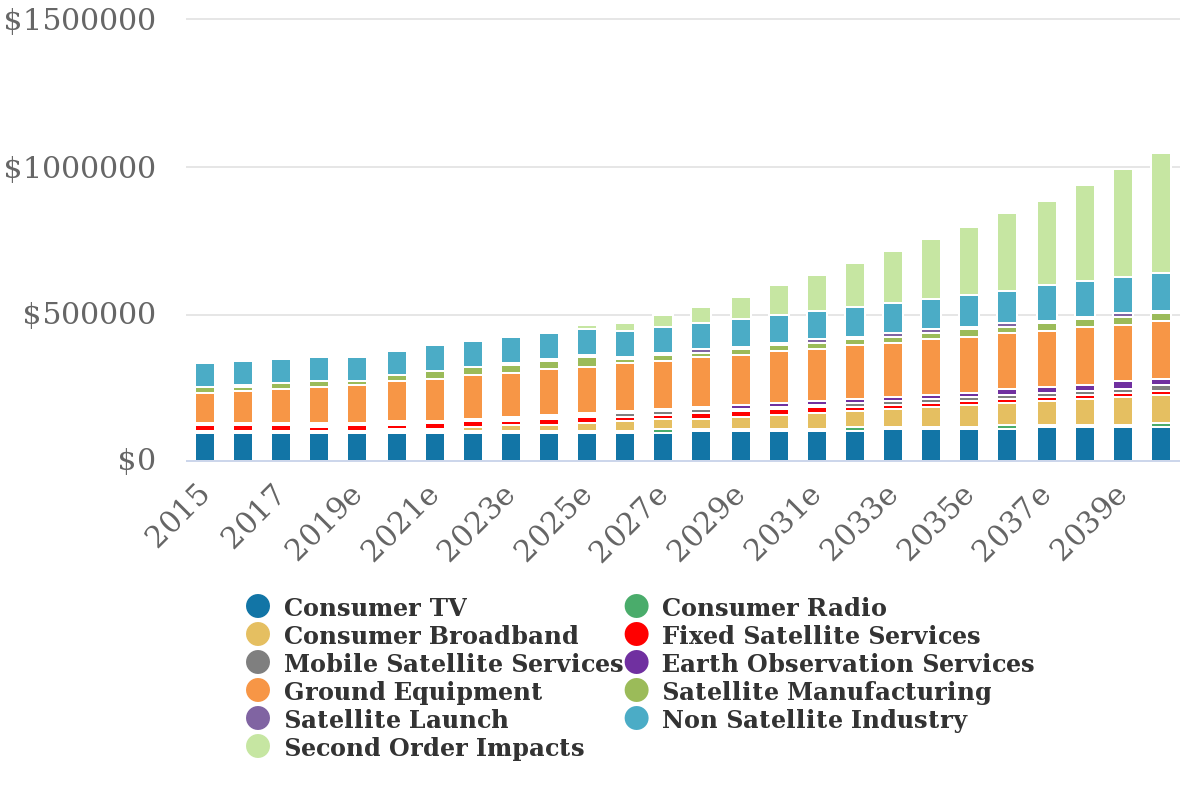
\includegraphics[scale=0.29]{images/morganstanley.png}
\caption{Global Market Trend according to Morgan Stanley.} \label{morgangraph}
\end{figure}
A report by Antrix and PwC, it is stated that the indian space sector can become a $\$$50 Billion industry, or about one per cent of India's projected $\$5$ Trillion economy, by 2024 from the current $\$7$ billion, according to a report by the Antrix and PwC.
\begin{figure}[H]
\centering
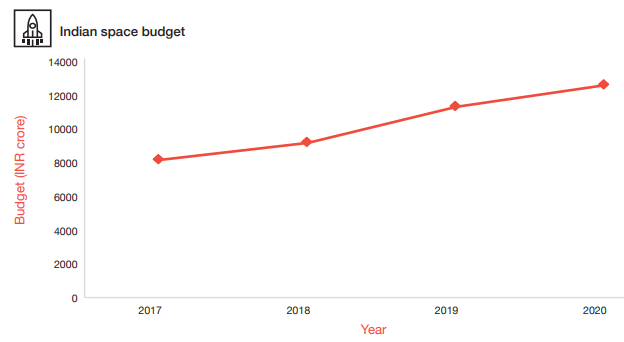
\includegraphics[scale=1]{images/pwc.png}
\caption{Indian Space Budget over the years.} \label{pwc}
\end{figure}
\subsection{Objective}
The development in the field of space technology is constantly increasing as shown in the aforementioned studies.
Such being the case, many students are showing interest to learn more and more about space technology and its related concepts. Considering all such possibilities, we have come up with an idea to develop a learning tool beneficial to learn more about Orbital Mechanics 
The main objectives of this project are as follows:
\begin{enumerate}
\item Design and develop a software to learn concepts and  solve Problems related orbital mechanics to understand the basics.
\item Provide a user friendly learning tool such that the user can operate even with the minimum knowledge about the concepts of orbital mechanics.
\item Help user to visualize the virtual view of the space mission.
\item Motivate the new comers to learn more abut the space studies. 
\end{enumerate}
\subsection{Front End Development}
\subsubsection{Introduction}
Front-end development deals with the Graphical User-Interface aspect of the software. It is the key developmental process that defines how the user experiences the features we have developed. The interface between the user and the back end code is GUI. The inputs from the user is taken from the GUI. So the design must be intuitive and clear. There are many libraries that can be used to develop a GUI like PyQt, Pyside, Kivy, Tkinter, etc. In our case, we have opted for PyQt5, Pyside2 and designed GUI in Qt-Designer. Then linked the Back-End scripts through the Integrated Development Environment(IDE) by Microsoft i.e, Visual Studio Code.
\subsubsection{Home Page}
When the application opens the Home Page will load. In it, there is a Dropdown box containing all the features available, from which the user can choose which feature they want to use. When the user selects any of the features from the drop-down and clicks on the go button at the bottom, they are navigated to that screen where they can use the feature they selected. And then if they want to navigate back to the Home-Page they can click on the Home button provided at the top left corner of the screen. All the features are listed in the upper-mentioned table.
\begin{figure}[H]
\centering
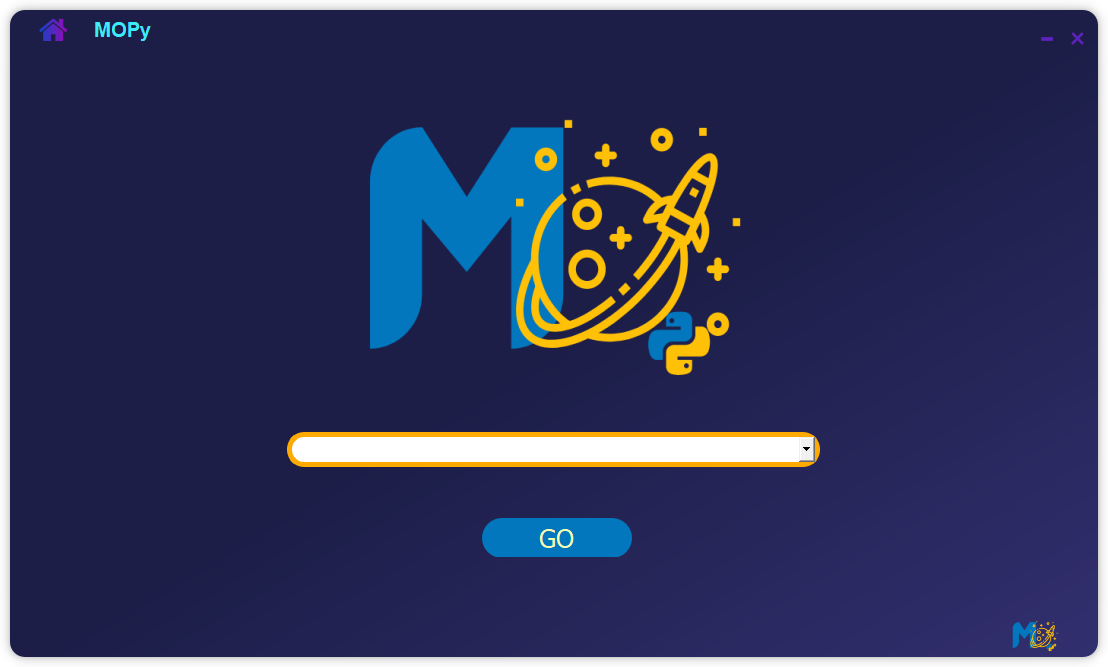
\includegraphics[scale=0.6]{images/homepage.png}
\caption{Home Page of MOPy} \label{home}
\end{figure}

\section{Details of the Features}
\subsection{Calculation of Orbital Elements}
This can convert state velocity vector into orbital elements and vice versa. The inputs are as follows
\begin{table}[H]
\centering
\begin{tabular}{@{}cl@{}}
\toprule
\multirow{2}{*}{Inputs} & State and Velocity Vectors            \\ \cmidrule(l){2-2} 
                                 & \multicolumn{1}{l}{Orbital Elements} \\ \midrule
\multicolumn{1}{r}{\multirow{2}{*}{Outputs}} & \multicolumn{1}{l}{Orbital Elements} \\ \cmidrule(l){2-2} 
\multicolumn{1}{r}{}           & State and Velocity Vectors            \\ \bottomrule
\end{tabular}\caption{Inputs and outputs for Calculation of Orbital Elements}
\end{table}
\begin{figure}[H]
\begin{floatrow}
\ffigbox{%
  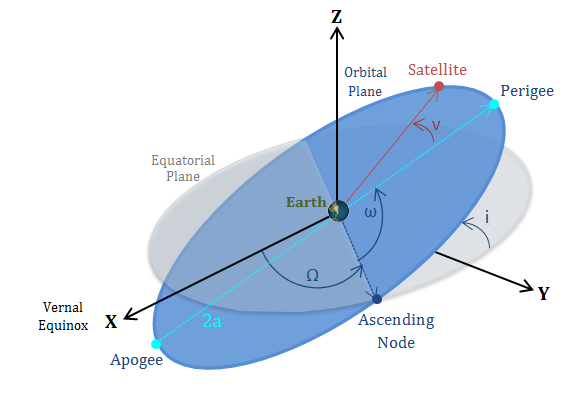
\includegraphics[scale=0.3]{images/COE.png}
}{
  \caption{Classical Orbital Elements} \label{COE}
}
\ffigbox{%
  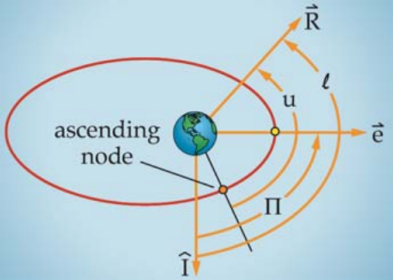
\includegraphics[scale=0.5]{images/AOE.png}
}{
  \caption{Alternate Orbital Elements} \label{AOE}
}
\end{floatrow}
\end{figure}

\large \hspace{-3em}\textbf{Classical Orbital Elements}
\normalsize
\begin{enumerate}
\item \textbf{Semi-major Axis($a$):} This is a constant that defines the size of the orbit. In Circular it is the radius of the circle. It is the longest diameter of an ellipse.
\begin{align}
a&= \dfrac{r_a+r_p}{2}\\
a&=\dfrac{h^2/\mu}{1-e^2}\\
where,\nonumber \\
&r_a = Radius\;of\;Apogee(F_1B)\nonumber\\
&r_p = Radius\;of\;Perigee(F_1A)\nonumber \\
&\mu = Standard\;Gravitational\;Parameter,\nonumber
\end{align}
\item \textbf{Eccentricity($e$):} This the parameter of the conic section which determines its shape. It is defined as the ratio of distance b/w two foci to the Major-axis.
\begin{align}
e&=\dfrac{c}{a}\\
e&=\frac{1}{\mu}\left[\left(\frac{v^2-\mu}{r}\right)\times \overrightarrow{r}-(\overrightarrow{r}.\overrightarrow{v})\times \overrightarrow{v}\right]\label{codeformecc} \\ 
where, \nonumber\\
r_a\;\&\;r_p &= Radius\;of\;Apogee\;\&\;Perigee\;respectively,\nonumber\\
\mu &= Standard\;Gravitational\;Parameter,\nonumber \\
\overrightarrow{v}\;\&\; v &= Velocity\;vector\;\&\;Magnitude\;of\;Velocity\;Vector\;at\;r,\nonumber \\
\overrightarrow{r}\;\&\;r &= Radius\;Vector\;\&\;Magnitude\;of\;Radius\;Vector.\nonumber 
\end{align}
\item \textbf{Inclination($e$)}: It is the tilt of the orbit w.r.t the equatorial plane, measured at ascending node. It can also be defined as the angle from $\hat{K}$ unit vector to the specific angular momentum vector $\vec{h}$.
\begin{align}
i &= \cos^{-1}\left(\dfrac{\overrightarrow{h}.\overrightarrow{K}}{|h|}\right)\\
where,\nonumber \\
\overrightarrow{h}&=Specific\;Angular\;Momentum, \nonumber \\
\overrightarrow{K}&=Unit\;Vector\;in\;Z\;direction, \nonumber  \\
|h|&=Magnitude\;of\;Specific\;Angular\;Momentum. \nonumber
\end{align}
\item \textbf{Right Ascension of Ascending Node($\Omega$):} RAAN horizontally orients the ascending node of the orbit w.r.t the Equatorial plane’s vernal equinox, measured in an equatorial plane This is not defined when the inclination is 0 or 180 degree. It lies between 0 to 360 degrees.
\begin{align}
\Omega &= \cos^{-1}\left(\dfrac{\overrightarrow{I}.\overrightarrow{n}}{|n|}\right)\\
where, \nonumber \\
\overrightarrow{n}&= Nodal\;vector \nonumber\\
It's\;the\;vector\;that\;&joins\;the\;ascending\;node\;and\;the\;descending\;node. \nonumber
\end{align}
\item \textbf{Argument of Perigee($\omega$):} Argument of Perigee defines the orientation of the ellipse in the orbital plane, as an angle measured from the ascending node to the periapsis measure in the direction of the spacecraft’s motion. This is not defined when inclination is 0 or 180 degree or eccentricity is 0. It lies between 0 to 360 degree.
\begin{align}
\omega &= \cos^{-1}\left(\dfrac{\overrightarrow{n}.\overrightarrow{e}}{|n||e|}\right)\\
where, \nonumber\\
\overrightarrow{e}&=Eccentricity Vector. \nonumber
\end{align}
\item \textbf{True Anomaly($\nu$):} True Anomaly defines the position of the spacecraft w.r.t perigee. It’s the angle between the spacecraft and the perigee of the orbit. It lies between 0 to 360 degree. 
\begin{align}
\nu &= \cos^{-1}\left(\dfrac{\overrightarrow{e}.\overrightarrow{r}}{|e||r|}\right)\\
where,\nonumber\\
\overrightarrow{r}&=Radius Vector\nonumber
\end{align}
\end{enumerate}
\large \textbf{Alternate Orbital Elements}
\normalsize
\begin{enumerate}
\item \textbf{Longitude of Perigee($Pi$)} is the angle from the principle direction to perigee. This is used whenever inclination is either 0$^o$ or 180$^o$ as there is no ascending node. It's lies between $0^0$ to $360^0$. In the figure(\ref{AOE}) Longitude of perigee is represented as \enquote{$\Pi$}.
\begin{align}
\Pi = \cos^{-1}\left(\dfrac{\overrightarrow{I}.\overrightarrow{e}}{|e|}\right)
\end{align}
\item \textbf{True Longitude} is the angle from the principle direction to the spacecraft's position. This is used whenever there is no perigee and the the inclination is either $0^0$ or $180^0$. It's lies between $0^0$ to $360^0$. It lies between 0 to 360 degree. In the figure(\ref{AOE})True Longitude is represented as \enquote{$l$}
In the figure(\ref{AOE})True Longitude is represented as \enquote{$l$}. In the figure(\ref{AOE}) Longitude of perigee is represented as \enquote{$\Pi$}.
\begin{align}
l = \cos^{-1}\left(\dfrac{\overrightarrow{I}.\overrightarrow{r}}{|r|}\right)
\end{align}
\item \textbf{Argument of Latitude($u$)} is the angle from ascending to the spacecraft's position. This is used whenever a perigee is absent(i.e., e=0,Circular Orbit). It's lies between $0^0$ to $360^0$.\\
In the figure(\ref{AOE}) Argument of latitude is represented as \enquote{$u$}.
\begin{align}
u = \cos^{-1}\left(\dfrac{\overrightarrow{n}.\overrightarrow{r}}{|n||r|}\right)
\end{align}
\end{enumerate}
\subsection{2D and 3D Orbits}

Based on the inputs given the application can plot either 2D or 3D or both. If the inputs are just Semi major axis and eccentricity or Radius of perigee and apogee or, $r_1,\;v_1,\;\gamma_1$ then the resultant plot will be in the perifocal frame. If the inputs are state and velocity vector or orbital elements then the resultant will be a 3D orbit. 
\begin{table}[H]
\centering
\begin{tabular}{@{}cl@{}}
\toprule
\multirow{2}{*}{\textbf{Inputs}}                      & For 2D - $a,e/r_a,r_p/ r_1, v_1, \gamma_1$ \\ \cmidrule(l){2-2} 
                                             & For 3D - Orbital Elements, State Vectors   \\ \midrule
\multicolumn{1}{r}{\multirow{2}{*}{\textbf{Outputs}}} & Orbit in the Perifocal Frame               \\ \cmidrule(l){2-2} 
\multicolumn{1}{r}{}                         & Orbit in a virtual 3D Environment          \\ \bottomrule
\end{tabular}
\caption{I/O for 2D and 3D orbits}
\label{o23}
\end{table}
There are two ways to plot a orbit, if the plot is on a 2D plane, i.e., Perifocal Plane, the the trajectory equation can be used to plot it easily.
$$r=\dfrac{h^2/\mu}{1 - e\cos(\theta)}$$
If the plot is 3D then solving for the trajectory analytically can be tricky and expensive computing wise depending on the orbit. But, solving it numerically will yeild the orbit with wide range of accuracy depending on the numerical method. The method has mainly two properties to be considered for at this level, the computing speed and the accuracy. A good compromise between these both is desirable for most of the cases. In this case we need a ODE solver. Here are a few types of numerical methods:
\begin{enumerate}
\item Euler Method
\item Backward Euler Method
\item First-order Exponential integrator Method
\item Generalizations
\item Parallel-in-time Methods
\item Integrals over Infinite intervals
\end{enumerate} 
In a programming language based on these methods ODE solvers are written. The most popular ones are:
\begin{enumerate}
\item \textbf{lsoda} - This automatically selects a solver which is appropriate for the given equation.
\item \textbf{lsode} - Since lsoda turns out to be slow, then the DE might need a stiff solver(i.e., very small time steps), this will choose only the stiff solvers 
\item \textbf{ode23} -  Simultaneously uses fourth and fifth order RK formulas to make error estimates and adjust the
time step accordingly. For nonstiff ODEs
\item \textbf{ode45} - Uses simultaneously second and third order Runge Kutta formulas to make estimates of the
error, and calculate the time step size. Since the second and third order RK require less steps, ode23 is
“less expensive” in terms of computation demands than ode45, but is also lower order. Use for nonstiff
ODEs
\end{enumerate}
For MOPy lsoda is sufficient enough for now. So lsoda is used to solve for the acceleration vector. If the acceleration vector is solved twice then we obtailn the position vectors using which a 3D plot can be plotted. The acceleration vector is: 

$$Enter the acceleration vector$$

\subsection{Euler Angle}

The inputs for this are as in table(\ref{eadcm}). This code can be fed the model in 3D environment and the orientation of the model can be manipulated with this.
\begin{table}[H]
\centering
\begin{tabular}{@{}cl@{}}
\toprule
\multirow{2}{*}{\textbf{Inputs}}                      & Directional Cosine Matrix \\ \cmidrule(l){2-2} 
                                             & Euler Angles              \\ \midrule
\multicolumn{1}{r}{\multirow{2}{*}{\textbf{Outputs}}} & Euler Angles              \\ \cmidrule(l){2-2} 
\multicolumn{1}{r}{}                         & Directional Cosine Matrix \\ \bottomrule
\end{tabular}
\caption{I/O for conversion between Euler angle and DCM}
\label{eadcm}
\end{table}
Euler Angles:
	The Euler angles are three angles introduced by Leonhard Euler to describe the orientation of a rigid body with respect to a fixed coordinate system. They can also represent the orientation of a mobile frame of reference in physics or the orientation of a general basis in 3-dimensional linear algebra. Euler angles can be defined by elemental geometry or by composition of rotations (matrix).
	The three elemental rotations may be extrinsic (rotations about the axes xyz of the original coordinate system, which is assumed to remain motionless), or intrinsic (rotations about the axes of the rotating coordinate system XYZ, solidary with the moving body, which changes its orientation after each elemental rotation).Euler angles are typically denoted as $\psi, \theta, \phi$
\begin{figure}[H]
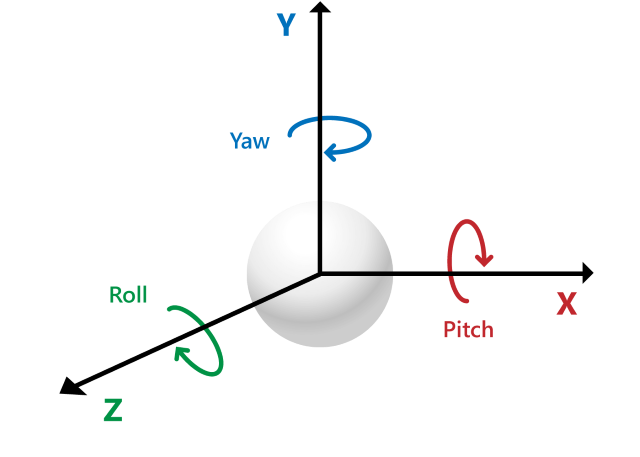
\includegraphics[scale=0.25]{images/EA1.png}
\caption{Euler Vector}
\end{figure}

\subsection{Sphere of Influence}
In this section, the user can either input the values or interact with the model in the 3D environment to see the corresponding output.
\begin{table}[H]
\centering
\begin{tabular}{@{}rl@{}}
\toprule
\multicolumn{1}{c}{\textbf{Inputs}} & Minor Body                     \\ \midrule
\multirow{2}{*}{\textbf{Outputs}}   & Radius of SOI in desired units \\ \cmidrule(l){2-2} 
                           & 3D visualization of sphere of influence in virtual environment                         \\ \bottomrule
\end{tabular}
\caption{I/O for Sphere of Influence}
\label{soi}
\end{table}
The sun is the dominant celestial body in the solar system. It has a mass of over 300,000 earths. The sun’s gravitational pull holds all the planets in its hold according to Newton’s law of gravity. However, near a given planet, the influence of its own gravity exceeds that of the sun. For example, at its surface the earth’s gravitational force is over 1600 times greater than the sun’s. The inversesquare nature of the law of gravity means that the force of gravity $F_g$ drops off rapidly with distance r from the center of attraction. If $F_{g0}$ is the gravitational force at the surface of a planet with radius $r_0$, then Figure 8.5 shows how rapidly the force diminishes with distance. At ten body radii, the force is 1$\%$ of its value at the surface. Eventually, the force of the sun’s gravitational field overwhelms that of the planet.

To estimate the planets Sphere of Influence, the three body problem system comprising of planet p of mass MiB\_ mass, the sun s and its mass MaB\_ mass with the distance between then being R and the equation on hand is:
\begin{align*}
r_{SOI}&=R\left(\dfrac{MiB\_ mass}{MaB\_ mass}\right)^{2/5}
\end{align*}

\begin{figure}[H]
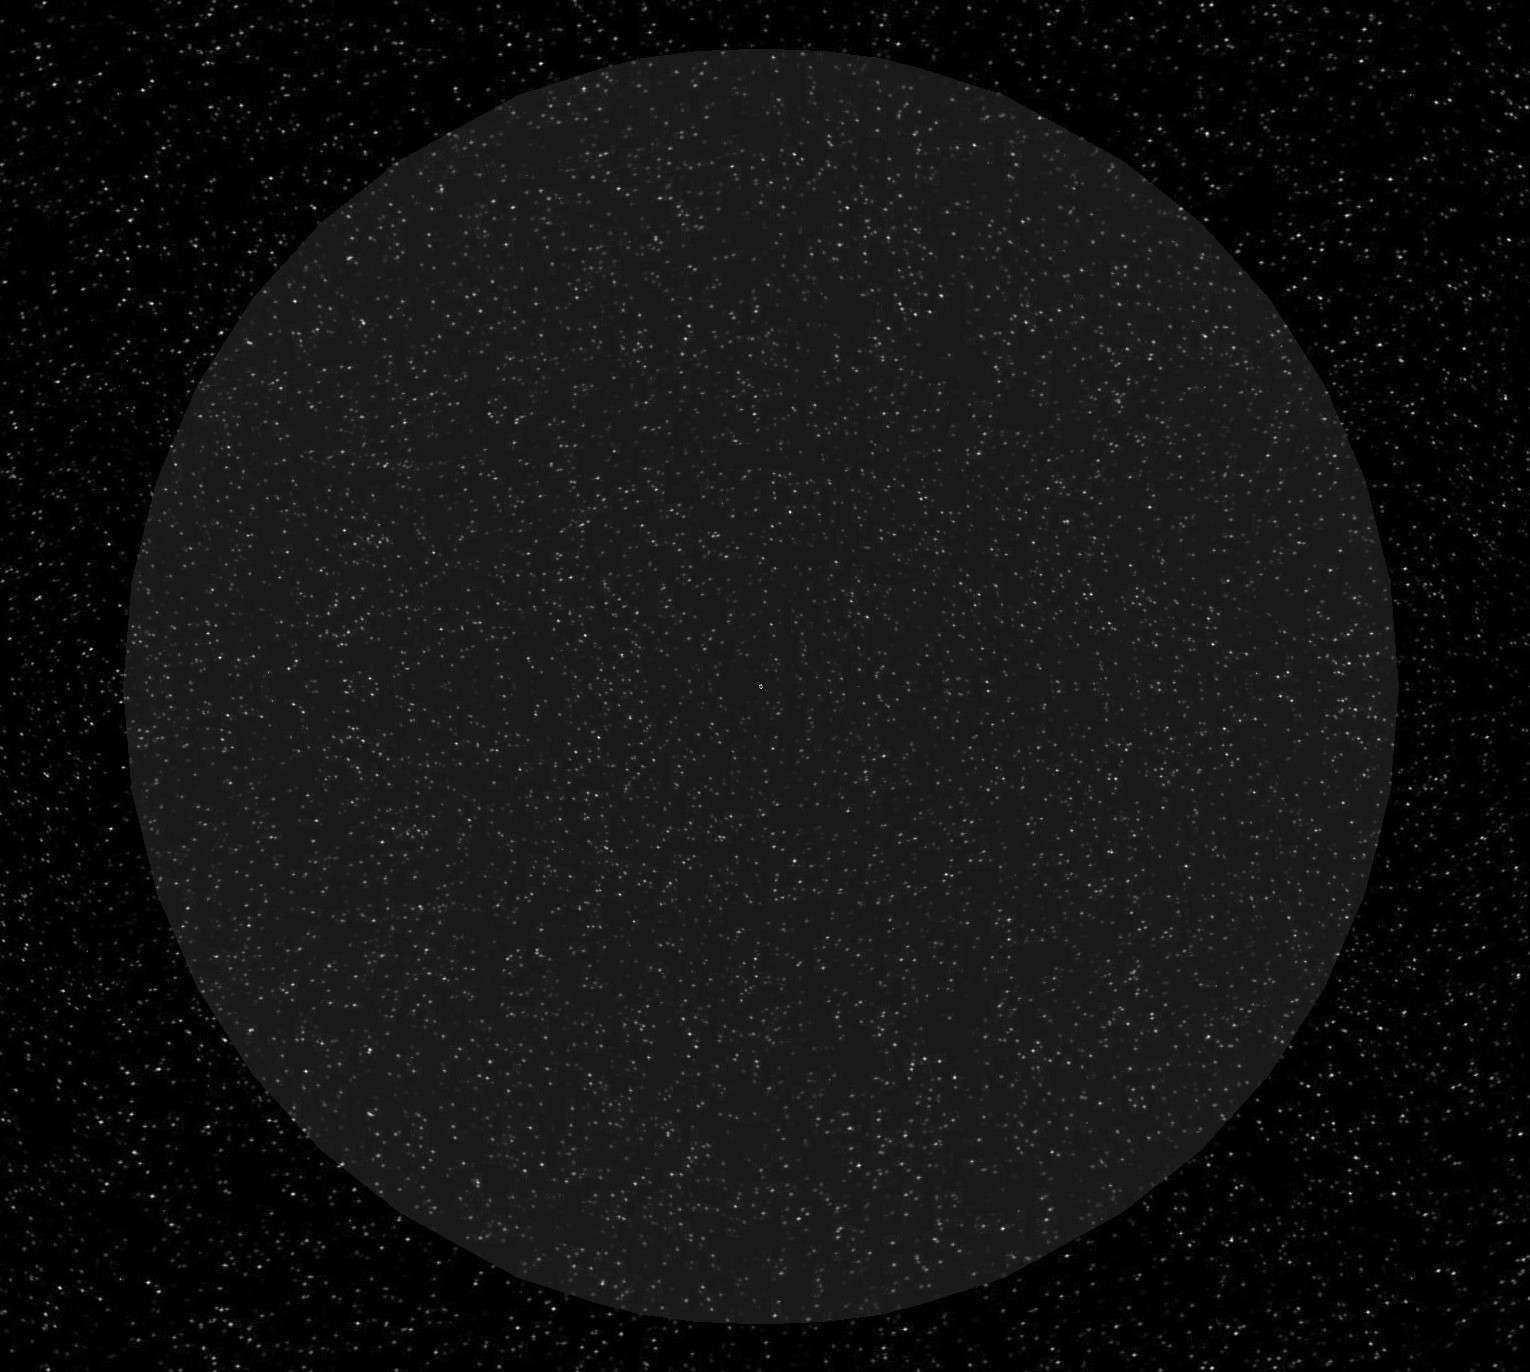
\includegraphics[scale=0.25]{images/soi.jpg}
\caption{Sphere of Influence of Earth, which is approx 140 times it's radius}
\end{figure}

\subsection{Orbital Transfer}
This feature simulates the orbital transfer using various numerical methods. For now, this can perform Hohmann Transfer. The Inputs and outputs are as in table(\ref{tab:ot})
\begin{table}[H]
\centering
\begin{tabular}{@{}cl@{}}
\toprule
\multicolumn{1}{c}{\textbf{Inputs}} & Minor Body, Major Body, Orbital parameters of both initial and final orbit.                     \\ \midrule
\multirow{2}{*}{\textbf{Outputs}}   & Values such as Radius of apogee, Radius of perigee, DeltaV, Time-period of the orbit etc \\ \cmidrule(l){2-2} 
                           & 3D visualization of desired orbital transfer \\ \bottomrule
\end{tabular}
\caption{I/O for Orbital transfer}
\label{tab:ot}
\end{table}
Transfer Orbit is nothing but the path followed by the satellite to travel from an initial orbit to final 
orbit or one planet to other planet. There are many types of transfer orbits in which most commonly used transfer 
is Hohmann Transfer because of its simplicity and its efficient to transfer.
Transfer orbits are:
\begin{enumerate}
\item \textbf{Hohmann Tranfer Orbit: }A Hohmann Transfer is a two-impulse(delta-v) elliptical transfer between two co-planar circular/elliptical orbits. The transfer orbit's apoapsis lies on the target orbit and the periapsis of transfer orbit lies on the initial orbit.The fundamental assumption behind the Hohmann transfer, is that there is only one major body which exerts a gravitational force on the body of interest, such as a satellite. This is most commonly used transfer method for transferring an earth-based satellite from a low orbit to say a geosynchronous orbit.
\begin{figure}[H]
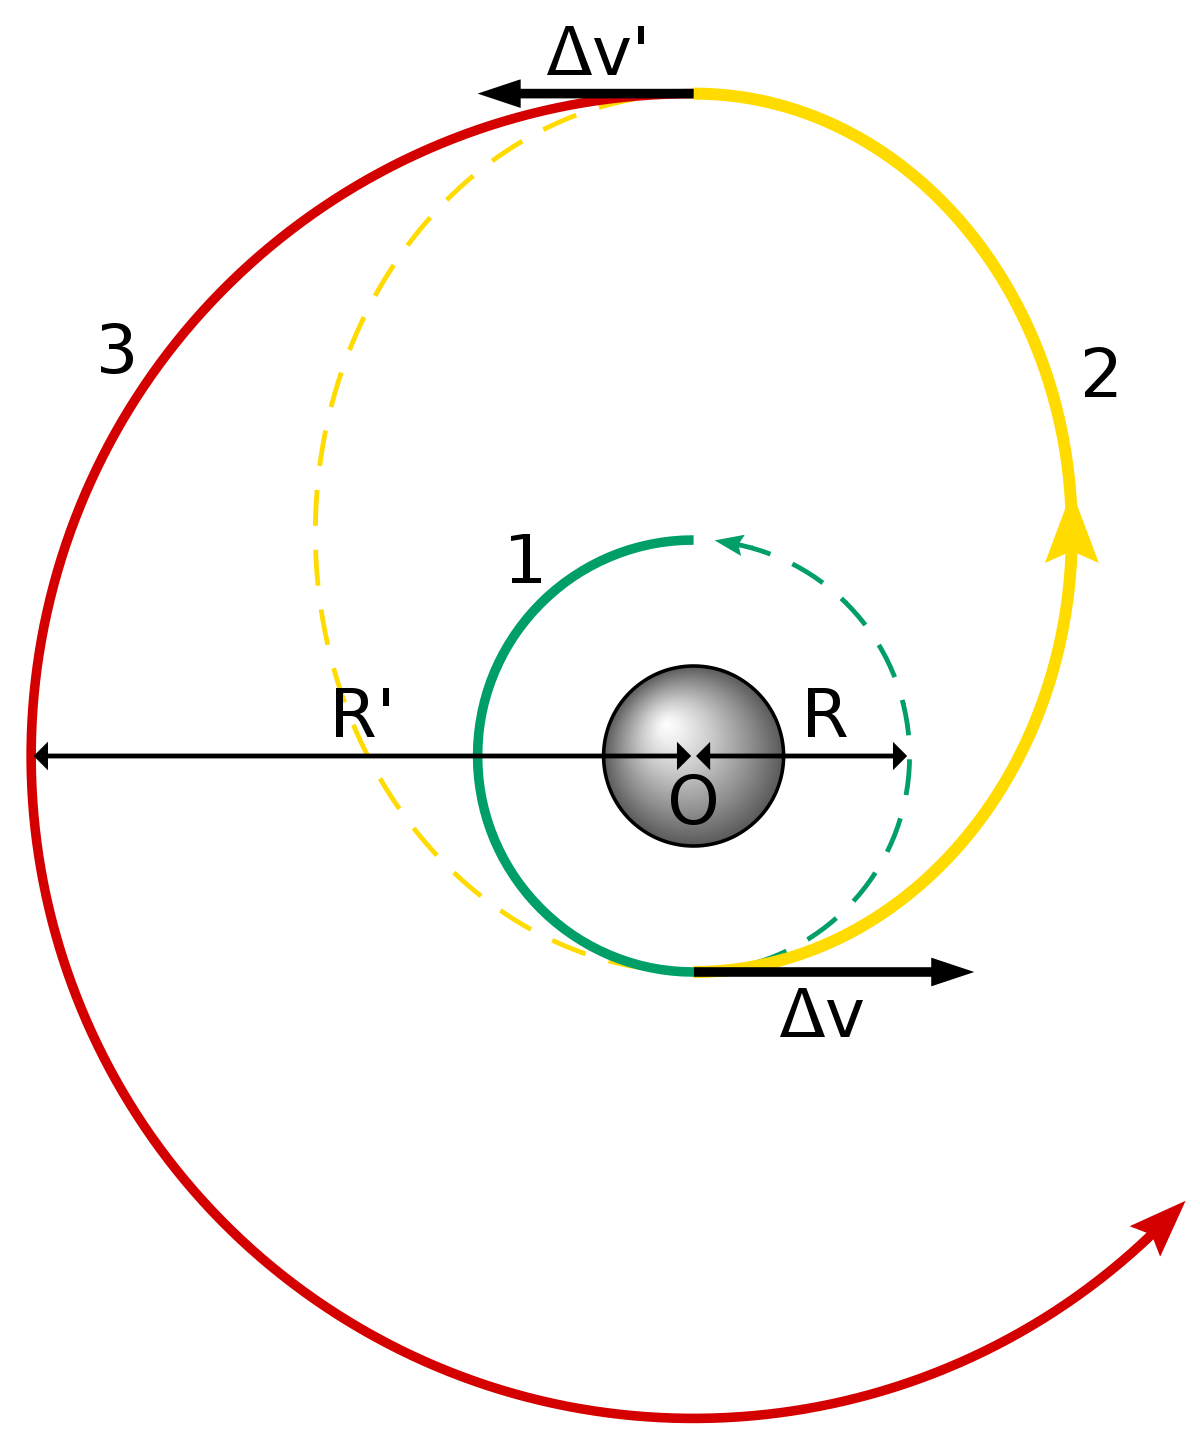
\includegraphics[scale=0.2]{images/ht.png}
\caption{Hohmann Transfer}
\end{figure}
\item \textbf{Bielliptical Transfer Orbit}: In the bi-elliptic transfer, the first transfer is a highly eccentric orbit with an apoapsis higher than the target orbit radius. Once the spacecraft has reached apoapsis, it performs a prograde burn raising its periapsis to the height of its target orbit. Finally, once it reaches periapsis, it performs an orbital insertion burn (Retrograde burn) to put it into a circular orbit. In some cases Bielliptical Transfer is preffered over Hohmann transfer because its
slight fuel efficint transfer.
\begin{figure}[H]
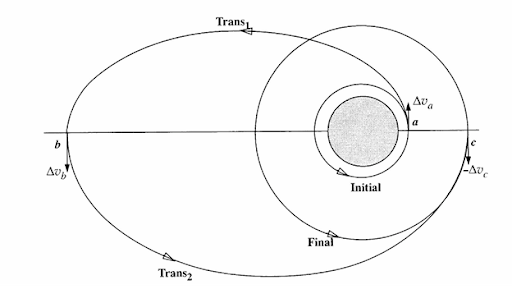
\includegraphics[scale=0.85]{images/bi.png}
\caption{Hohmann Transfer}
\end{figure}
\item \textbf{Low Energy Transfer Orbit:} A low energy transfer is a path in space to reach a target with very little consumption of fuel.
\item \textbf{Constant-Thrust Transfer Orbit:} In this transfer path the spacecraft's engine will be producing constant thrust through out the path. The spacecraft points straight towards the target with constant acceration till it reaches the target. 
\end{enumerate}
\subsection{Calculation of Julian Day}
In this section the user can choose between Gregorian calendar and Julian calendar and with the other inputs they can obtain the Julian day of the corresponding date. 
\begin{table}[H]
\centering
\begin{tabular}{@{}cl@{}}
\toprule
\textbf{Inputs}  & YYYY-MM-DD , hh:mm:ss, Type of calender \\ \midrule
\textbf{Outputs} & Julian-day  \\ \bottomrule                                              
\end{tabular}
\caption{I/O for Julian-day}
\label{tab:jd}
\end{table}
The Julian day is the continuous count of days since the beginning of the Julian period i.e., January 1, 4713 B.C. at 12 Noon, and is used primarily by astronomers for easily calculating elapsed days between two events.
To calculate a Julian Day there are many formulae, but the generalised formula is:\\
To convert from Gregorian calendar:
\begin{multline*}
JDN = \dfrac{1461\left(Y+4800+\dfrac{M-14}{12}\right)}{4}+\dfrac{367\left(M-2-12\dfrac{M-14}{12}\right)}{12} - \\
\dfrac{3\left( \dfrac{Y+4900+\dfrac{M-14}{12}}{100}\right))}{4}+D-32075
\end{multline*}
To convert from Julian Calendar:
$$JDN = 367 \times Y - \dfrac{7 \left( Y+5001+\dfrac{M-9}{7}\right)}{4}+\dfrac{275M}{9}+D+1729777$$
Once the Julian Day Number is obtained the time is taken into account. So, The Julian day becomes:
$$JD = JDN+\dfrac{HH-12}{24}+\dfrac{MM}{1440}+\dfrac{SS}{86400}$$
\subsection{Calculation of Parameters of the Orbit}
The user can obtain various parameters by giving the details that they know of. If necessary they can plot the orbit too.
\begin{table}[H]
\centering
\begin{tabular}{@{}rl@{}}
\toprule
\multicolumn{1}{c}{\textbf{Inputs}} & $a,e/r_a, r_p/r_1,\;v_1,\;\gamma_1$/ Orbital Elements/State and velocity vectors \\ \midrule
\multirow{2}{*}{\textbf{Outputs}}   & $\mu,\;,h\;,\epsilon$, Forces and Velocity at significant position               \\ \cmidrule(l){2-2} 
                           & Mean Motion, Time Period                                                         \\ \bottomrule
\end{tabular}
\caption{I/O for Various Parameters of the Orbit}
\label{vpco}
\end{table}
The Semi major axis ,Eccentricity, Radius of perigee, Radius of apogee, Specific mechanical energy, Specific angular momentum, Time period , Mean motion, Velocity at perigee, Velocity at apogee, Gravitational force at perigee, Gravitational force at apogee, Semi-latus rectum, Velocity at semi-latus rectum, Escape velocity at perigee and Escape velocity at apogee all these parameters can be calculated. These parameters can be calculated at any given point of time in the ongoing mission.
The major formula used in it are:\\

% Please add the following required packages to your document preamble:
% \usepackage{multirow}
\begin{table}[H]
\centering
\begin{tabular}{ccc}
\
\textbf{Circular and Elliptical}           & \textbf{Parabolic}               & \textbf{Hyperbolic}                             \\ \hline
\multicolumn{3}{c}{$\mu=G\times M_{Major}$}                                                                                                                               \\ 
\multicolumn{1}{c|}{$r_p=a\times (1-e)$}                        & \multicolumn{1}{c|}{\multirow{2}{*}{$l=2\times r_p$}} & $\theta_\infty = \cos^{-1}(\dfrac{1}{e})=\beta$ \\
\multicolumn{1}{c|}{$r_a=a\times (1+e)$}                        & \multicolumn{1}{c|}{}                                 & $\delta = 2\sin(\dfrac{1}{e})$                  \\
\multicolumn{1}{c|}{$\epsilon = \dfrac{-\mu}{2a}$}              & \multicolumn{1}{c|}{$0$}                              & $h=\sqrt{\mu a(e^2-1)}$                         \\
\multicolumn{1}{l|}{}                                           & \multicolumn{1}{l|}{}                                 & \multicolumn{1}{l}{}                            \\
\multicolumn{1}{c|}{$h=\sqrt{r_p\times(1+e)\mu}$}               & \multicolumn{1}{c|}{$h=\sqrt{2\mu r_p}$}              & $b=ae\sin(\theta_\infty)=\Delta$                \\
\multicolumn{1}{l}{}                                            & \multirow{2}{*}{$F_g=\dfrac{GMm}{r^2}$}               & \multicolumn{1}{l}{}                            \\
                                                                &                                                       &                                                 \\
\multicolumn{1}{c|}{$V= \sqrt{\dfrac{2\mu}{r}-\dfrac{\mu}{a}}$} & \multicolumn{1}{c|}{$V_r=\sqrt{\dfrac{2\mu}{r}}$}     & $V_\infty=e\mu\sin(\theta_\infty)/h$            \\
\multicolumn{1}{c|}{$T = \sqrt{\dfrac{4\pi^2}{\mu}\times a^3}$} & \multicolumn{1}{c|}{}                                 & $\epsilon=\dfrac{\mu}{2a}$                      \\
\multicolumn{1}{c|}{$n = \dfrac{2 \pi}{T}$}                     & \multicolumn{1}{c|}{}                                 & $l=\dfrac{-b^2}{a}$                             \\
\multicolumn{1}{c|}{$l=a\times(1-e^2)$}                         & \multicolumn{1}{c|}{}                                 & $r_p,r_a = \dfrac{h^2/\mu}{1 \pm e}$           
\end{tabular}
\caption{Formulae for Various parameters}
\label{tab:vpco}
\end{table}
\subsection{Sensitivity Analysis}
This calculates the value of the error that rises up if the initial value is very slightly different than what it is supposed to be. \\
\begin{table}[H]
\begin{tabular}{@{}cl@{}}
\toprule
\textbf{Input}  & State Vector, Velocity Vector and two delta-v with slight difference                                                                      \\ \midrule
\textbf{Output} & \begin{tabular}[c]{@{}l@{}}Percentage difference caused to the final orbit parameters due to slight \\ difference in delta-v\end{tabular} \\ \bottomrule
\end{tabular}\caption{I/O for Sensitivity Analysis}
\end{table}
The analysis is done to know what is the effect, if small error occurs in position and velocity at the maneuver point while the space mission is on the trajectory. There is a derived formula to calculate the sensitivity analysis from which change in position and velocity can be obtained in terms of percentage . This helps in analysing the position and velocity tolerance of any particular mission and design accordingly.
$$\dfrac{\delta R_2}{R_2}=\dfrac{2}{1-\dfrac{R_1\left[V_D^{v}\right]^2}{2\mu_{sun}}}\left(\dfrac{\mu_1}{V_D^{v}v_\infty r_p}\dfrac{\delta r_p}{r_p}+\dfrac{v_\infty+\dfrac{2\mu_1}{r_pv_\infty}}{V_D^{v}}\dfrac{\delta v_p}{v_p}\right)$$
\subsection{Position of One Spacecraft Relative To Another}
Based on the inputs of the user the relative velocity and orbit can be visualized in this section.
\begin{table}[H]
\begin{tabular}{@{}cl@{}}
\toprule
\textbf{Input}  & Major Body, State Vector and Velocity Vector of Minor Body    \\ \midrule
\textbf{Output} & Graph Showing the Minor bodies in the orbit around Major Body \\ \bottomrule
\end{tabular}\caption{I/O for Position of One Spacecraft Relative To Another}
\end{table}

In situations like a rendezvous maneuver the relative motion between the space vehicles is utilised. This can be done in two different ways, utilising the algorithm to calculate the relative orbit or utilise the camera viewpoint and plotting as the orbit propagates with the camera fixed on one of the spacecraft.
\subsection{Lagrangian Points}
The Lagrangian points are points near two large orbiting bodies, the two objects exert an unbalanced gravitational force at a point, altering the orbit of whatever is at that point. At the Lagrange points, the gravitational forces of the two large bodies and the centrifugal force balance each other, The inputs and outputs are as follows.
\begin{table}[H]
\begin{tabular}{@{}cc@{}}
\toprule
\textbf{Input}  & Major Body, Minor Body and Distance Between them           \\ \midrule
\textbf{Output} & Lagrangian points polar coordinates and Graph showing them \\ \bottomrule
\end{tabular}\caption{I/O for Lagrangian Points}
\end{table}
    Lagrange Points are positions in space around the planet/star, where the gravitational forces of two body like the Sun and the Earth produce enhanced regions of attraction and repulsion. These can be used by spacecraft to reduce fuel consumption required to remain in position. At these points gravitational pull of two large masses precisely equals the centripetal force required for a small object to move with them.
    
    These points are named in honor of Italian-French mathematician Josephy-Louis Lagrange. There are five Langrengian points around the planet/satr, where a small mass can orbit in a constant pattern with two larger masses.  This mathematical problem, known as the "General Three-Body Problem" was considered by Lagrange in his prize winning paper (Essai sur le Problème des Trois Corps, 1772).     Of the five Lagrange points, three are unstable and two are stable. The unstable Lagrange points - labeled L1, L2 and L3 - lie along the line connecting the two large masses.The three of them lie along the line connecting the two large bodies.
The stable Lagrange points - labeled L4 and L5 - form the apex of two equilateral triangles that have the large masses at their vertices. L4 leads the orbit of earth and L5 follows.

\section{Database Management System}
\subsection{CRUD File Operations}
\begin{lstlisting}[language=python, caption=db.py]
# import sqlite in ide 
import sqlite3

# Create a database or connect to one 
conn= sqlite3.connect('appdatabase.db')

# Create a Cursor
c= conn.cursor()

# Creat a table
c.execute(""" CREATE TABLE table_name( 
        column_name datatype,
        column_name datatype
     )""")

# Insert data into table
x = [('column 1', 'column 2')
     ('column 1', 'column 2')
    ]
c.executemany( "INSERT INTO table_name VALUES(?,?)",x)

#Retrieve or read data 
c.execute("SELECT * FROM table_name")
print(c.fetchall())

# commit data to the database
conn.commit()
\end{lstlisting}

\section{Conclusion}
The outcome of the project is the lessons we learnt during the project. Communication is the key for collaborative work. This is one of the main aspect that we learned during this project. The other aspects that we were able to learn are:
\begin{enumerate}
\item Project Management
\item Time Management
\item Prioritize the list that is at hand based on various parameters
\end{enumerate}

\section{Future Scope}
\hspace{4em}MOPy is a open source application with GNU - GPL v3 License, with this anyone who is interested in using this application can freely download and use it, and even modify the contents to their requirements. If they wish to contribute to this application they can fork the repository on GitHub[3] and add their contribution by sending a pull request. The reason GNU-GPL v3 license is used is that we aim to keep a quality control to the features that gets added to the application. We are always open to contributors.

There is a list of features with corresponding priorities that are planned to be added down the line. This will be constantly updated indefinitely. And if the user is not able to add a feature then they can request a feature that would be added to the list with a appropriate priority. There is discord server in which anyone can join and hold discussions with other participants. Contributors can hold discussions about the feature they are planning to add, others can discuss about the concepts and request features to be added. 

As of now this runs on Windows only. This could be made to run on other platforms and even as a web application which would negate the need of a moderately powerful hardware. The database could be expanded with much more data than present.

This entire code can be converted into a library that anyone can download from PyPI. This would enable the user to utilize the features directly from the command line or their python projects. This would simplify their projects.

\appendix
\section{Code for the Features}
\subsection{Calculation Of Orbital Elements}
\begin{lstlisting}[language=python, caption=CoOE.py]
from numpy.linalg import norm
from numpy import dot, pi, cross, multiply as multi
from math import acos

class Calculate:
    I = [1, 0, 0]
    J = [0, 1, 0]
    K = [0, 0, 1]
    G = 6.67e-20 #units are in km3 kg-1 s-2

    @classmethod
    def muvalue(cls, major_body):
        major_body_list = pandas.read_csv("Major_and_Minor_Bodies.csv")
        major_bodies = list(major_body_list.Major_Body)
        major_bodies_mass = list(major_body_list.Mass)
        major_bodies_radius = list(major_body_list.Radius)        
        sel_major_body = major_bodies.index(major_body)
        major_body_mass = major_bodies_mass[sel_major_body]
        major_body_radius = major_bodies_radius[sel_major_body]
        mu = cls.G * major_body_mass
        return [mu, major_body_radius]
    
    @classmethod
    def correct_ohm(cls, ohm, n_vec):
        if n_vec[0] > 0 and n_vec[1] > 0: 
            print("This is a Prograde Elliptical Orbit and is in first Quadrant.")
            if ohm >90:
                ohm -= 360
        elif n_vec[0] < 0 and n_vec[1] > 0:
            print("This is a Retrograde Elliptical Orbit and is in second Quadrant.")
            if ohm > 180:
                ohm -= 360
        elif n_vec[0] < 0 and n_vec[1] < 0:
            print("This is a Retrograde Elliptical Orbit and is in Third Quadrant.")
            if ohm < 180:
                ohm -= 360
        elif n_vec[0] > 0 and n_vec[1] < 0:
            print("This is a Prograde Elliptical Orbit and is in fourth Quadrant.")
            if ohm < 90:
                ohm -= 360
        return ohm

    @classmethod
    def other_var(cls, pos_vec, vel_vec):
        h_vec = cross(pos_vec, vel_vec)
        n_vec = cross(cls.K,h_vec)
        return [h_vec, n_vec]

    @classmethod
    def OE(cls, pos_vec, vel_vec, mu):
        [h_vec, n_vec] = Calculate.other_var(pos_vec, vel_vec)
        e_vec = (multi((norm(vel_vec)*norm(vel_vec)-(mu/norm(pos_vec))),pos_vec)- multi(dot(pos_vec,vel_vec),vel_vec))/(mu)
        call.ecc_o.setText(str(norm(e_vec)))
        inc = (acos((dot(h_vec, cls.K))/norm(h_vec))) * 180/pi
        call.inc_o.setText(str(inc))
        sma = 1/((2/norm(pos_vec))-((norm(vel_vec)*norm(vel_vec))/mu))
        call.sma_o.setText(str(sma))
        return [sma, inc, e_vec]
    
    @classmethod
    def ACOE(cls, pos_vec, vel_vec, e_vec, inc):
        [h_vec, n_vec] = Calculate.other_var(pos_vec, vel_vec)
        if inc != 0 or 180 and norm(e_vec) > 0: #Nothing is Zero/180
            ohm = (acos((dot(cls.I,n_vec))/norm(n_vec)))
            ohm = Calculate.correct_ohm(ohm, n_vec)
            call.ohm_o.setText(str(ohm))
            nu = (acos((dot(e_vec,pos_vec))/(norm(e_vec)*norm(pos_vec))))
            call.nu_u_o.setText(str(nu))
            omega = (acos((dot(n_vec,e_vec))/multi(norm(n_vec),norm(e_vec))))
            call.omega_l_o.setText(str(omega))
            return [ohm, omega, nu]
        elif inc == 0 or 180: #Inclination is Zero
            if norm(e_vec) > 0: #Elliptical Orbit
                nu = (acos((dot(e_vec,pos_vec))/(norm(e_vec)*norm(pos_vec))))
                call.nu_u_o.setText(str(nu))
                Long_of_peri_pi = acos(dot(cls.I,e_vec)/(norm(cls.I)*norm(e_vec)))
                return [Long_of_peri_pi, nu]
            elif norm(e_vec) == 0: #Circular Orbit
                Tr_long_l = acos(dot(cls.I,pos_vec)/(norm(pos_vec)*norm(cls.I)))
                return [Tr_long_l]
        elif norm(e_vec) == 0: #Circular orbit with inclination non-zero/pi
            Arg_of_lattitude_u = acos(dot(n_vec,pos_vec)/(norm(n_vec)*norm(pos_vec)))
            return [Arg_of_lattitude_u]

    @classmethod
    def possibility(cls, major_body, pos_vec, vel_vec):
        [mu, major_body_radius] = Calculate.muvalue(major_body)
        pos = norm(pos_vec)
        vel = norm(vel_vec)
        sma = 1/((2/pos)-(vel*vel/mu))
        e_vec = (multi((norm(vel_vec)*norm(vel_vec)-(mu/norm(pos_vec))),pos_vec)- multi(dot(pos_vec,vel_vec),vel_vec))/(mu)
        r_peri = sma*(1-norm(e_vec))
        if r_peri <= major_body_radius:
            print("The Orbit is not possible as radius of perigee is less than radius of the major Body")
            return False
        return True
\end{lstlisting}

\subsection{Euler Angles}
\begin{lstlisting}[language=python, caption= EA.py]
from math import *
from numpy import *

class EA():

    def RxRyRz(pitch_theta, roll_phi, yaw_si):
        Rx = matrix([[ 1, 0 , 0 ],
                        [ 0, cos(roll_phi),sin(roll_phi)],
                        [ 0,-sin(roll_phi), cos(roll_phi)]])
        
        Ry = matrix([[ cos(pitch_theta), 0,-sin(pitch_theta)],
                        [ 0 ,1, 0],
                        [sin(pitch_theta), 0, cos(pitch_theta)]])
        
        Rz = matrix([[ cos(yaw_si), sin(yaw_si), 0 ],
                        [-sin(yaw_si), cos(yaw_si) , 0 ],
                        [ 0, 0, 1]])
        return [Rx, Ry, Rz]

    def DCMtoEA(DCM, order):
        if order=='321':
            theta=-asin(DCM[0][2])
            phi=atan(DCM[1][2]/DCM[2][2])
            si=atan(DCM[0][1]/DCM[0][0])
        elif order=='123':
            theta=asin(DCM[2][0])  
            phi=atan(DCM[2][1]/DCM[2][2])
            si=atan(DCM[1][0]/DCM[0][0])
        elif order=='132':
            theta=atan(DCM[2][0]/DCM[0][0])
            phi=atan(DCM[1][2]/DCM[1][1])
            si=-asin(DCM[1][0])
        elif order=='312':
            theta=atan(DCM[0][2]/DCM[2][2])
            phi=asin(DCM[1][2])
            si=atan(DCM[1][0]/DCM[1][1])
        elif order=='213':
            theta=atan(DCM[2][0]/DCM[2][2])
            phi=-asin(DCM[2][1])
            si=atan(DCM[0][1]/DCM[1][1])
        elif order=='231':
            theta=atan(DCM[0][2]/DCM[0][0])
            phi=atan(DCM[2][1]/DCM[1][1])
            si=asin(DCM[0][1])
        return [theta, si, phi]

    def EAtoDCM(theta, si, phi, order):
        [Rx, Ry, Rz] = EA.RxRyRz(theta, si, phi)
        if order=='321':
            RxRy = dot(Rx,Ry)
            return (dot(RxRy,Rz))
        elif order == '123':
            x = Rx(phi*pi/180)
            y = Ry(theta*pi/180)
            z = Rz(si*pi/180)
            zy = dot(z,y)
            return (dot(zy,x))
        elif order == '213':
            x = Rx(phi*pi/180)
            y = Ry(theta*pi/180)
            z = Rz(si*pi/180)
            zx = dot(z,x)
            return (dot(zx,y))
        elif order == '312':
            x = Rx(phi*pi/180)
            y = Ry(theta*pi/180)
            z = Rz(si*pi/180)
            yx = dot(y,x)
            return (dot(yx,z))
        elif order == '132':
            x = Rx(phi*pi/180)
            y = Ry(theta*pi/180)
            z = Rz(si*pi/180)
            yz = dot(y,z)
            return (dot(yz,x))
        elif order == '231':
            x = Rx(phi*pi/180)
            y = Ry(theta*pi/180)
            z = Rz(si*pi/180)
            xz = dot(x,z)
            return (dot(xz,y))
        else:
            return ('No transformation matrix')

order = '321' #input("Enter the order:")
DCM = [[0.6405, 0.75319, -0.15038],[0.76736, -0.63531, 0.086824],[-0.030154, -0.17101, -0.98481]]
print(EA.DCMtoEA(DCM,order))

print(EA.EAtoDCM(8.6489  * 180/pi, 49.619 * 180/pi, -5.039 * 180/pi, order))
\end{lstlisting}

\subsection{Sphere of Influence}
\begin{lstlisting}[language=python, caption=SoI]
from math import *
import numpy as np
import matplotlib.pyplot as plt
from mpl_toolkits.mplot3d import Axes3D
import sqlite3

def SoI(MiB_mass, MiB_radius, r_maj_to_min):
    MaB_mass = 1.989e30
    rSOI = (r_maj_to_min*(MiB_mass/MaB_mass)**(2/5))
    return [rSOI, rSOI/MiB_radius]
\end{lstlisting}

\subsection{Calculation of Julian Day}
\begin{lstlisting}[language=python, caption=CJSD.py]
from math import *
class JulianDay():

    @classmethod
    def tb_method(cls,year, month, day, hour, minutes, seconds, accuracy):
        if 1901 <= year <= 2099:
            JDN = 367 * year + int((7 * (year + int((month + 9)/12)))/4) + int(275 * month/9) + day + 1721013.5
            UT = hour + round((minutes/60), accuracy) + round((seconds/3600), accuracy)
            JD = JDN + UT/24
            return [JDN, JD]
        else:
            #manju you can set limits when this option is selected between 1901 and 2099
            print("Not Possible from this method")

    @classmethod
    def julian_day(cls,year, month, day, hour, minutes, seconds, accuracy,type_of_calender):
        if type_of_calender == "Gregorian":
            #julian day number from Gregorian calender date
            JDN = int((1461 * (year + 4800 + (month - 14)/12))/4) + int((367 * month - 2 - 12 * ((month - 14)/12))/12) - int((3 * ((year + 4900 + (month - 14)/12)/100))/4) + day - 32075
        elif type_of_calender == "Julian":
            #julian day number from julian calender date
            JDN = 367 * year - int((7 * (year + 5001 + (month - 9)/7))/4) + int((275 * month)/9) + day + 1729777
        #JDN to JD
        JD = JDN + round(((hour - 12)/24),accuracy) + round((minutes/1440), accuracy) + round((seconds/86400), accuracy)
        return [JDN, round(JD, accuracy)]

\end{lstlisting}

\subsection{Calculation of Various Parameters of the Orbit}
\begin{lstlisting}[language=python, caption=VPCO]
import numpy as np
from math import *

class GlobalCalculation():
    I = [1, 0, 0]
    J = [0, 1, 0]
    K = [0, 0, 1]
    G = 6.67e-20 #units are in km3 kg-1 s-2

    @classmethod
    def force_at_this_point(cls, r, major_body_mass, minor_body_mass):
        F_r = cls.G * major_body_mass * minor_body_mass / r ** 2
        return F_r


# all the units should be km
class CalculateCircularElliptical:
    I = [1, 0, 0]
    J = [0, 1, 0]
    K = [0, 0, 1]
    G = 6.67e-20 #units are in km3 kg-1 s-2
    def __init__(self, major_body):
    
        self.major_body = major_body
        return

    @classmethod
    def semiecc(cls, sma, mag_e, major_body):
        r_per = sma * (1 - mag_e)
        r_apo = sma * (1 + mag_e)
        [mean_motion, T_period, mag_h, sme, slr] = CalculateCircularElliptical.orb_const(r_per, sma, mag_e, major_body)
        return [r_per, r_apo, mean_motion, T_period, mag_h, sme, slr]
    
    @classmethod
    def perapo(cls, r_per, r_apo, major_body):
        sma = (r_per + r_apo)/2
        mag_e = (r_apo - r_per)/(r_apo + r_per)
        [mean_motion, T_period, mag_h, sme, slr] = CalculateCircularElliptical.orb_const(r_per, sma, mag_e, major_body)
        return [mag_e, sma, mean_motion, T_period, mag_h, sme, slr]
    
    @classmethod
    def orb_const(cls, r_per, sma, mag_e, major_body):
        major_body_mass = 5.972e24 #self.major_body * 1
        mu = cls.G * major_body_mass
        slr = sma*(1-mag_e**2)
        mag_h = (r_per*(1+e)*mu)**0.5
        T_period = sqrt(((4*pi**2)/mu)*sma**3)
        mean_motion = T_period/(2*pi)
        sme = -mu/(2* sma)
        return [mean_motion, T_period, mag_h, sme, slr]
    
    @classmethod
    def time_since_periapsis(cls, mag_e, theta, T_period):
        E_anomly = 2 * atan((sqrt((1 - mag_e)/(1 + mag_e)) * tan(theta/2)))
        M_anomly = E_anomly - mag_e * sin(E_anomly)
        t_since_perigee = T_period * M_anomly/(2*pi)
        return t_since_perigee
    
    @classmethod
    def velocity_at_any_point(cls, sma, r, major_body):
        major_body_mass = major_body * 1
        mu = cls.G * major_body_mass
        v_point = sqrt(((2 * mu)/r) - (mu/sma))
        return v_point

class CalculateParabola():
    I = [1, 0, 0]
    J = [0, 1, 0]
    K = [0, 0, 1]
    G = 6.67e-20 #units are in km3 kg-1 s-2

    @classmethod
    def const_values(cls, r_per, major_body):
        major_body_mass = major_body * 1
        mu = major_body_mass * cls.G
        slr = 2 * r_per
        v_per = sqrt((2*mu)/r_per)
        mag_h = sqrt(mu*r_per * 2)
        return [slr, v_per, mag_h]

    @classmethod
    def velocity_at_any_point(cls, r, major_body):
        major_body_mass = major_body * 1
        mu = major_body_mass * cls.G
        v = sqrt((2*mu)/r)
        return v
    
class CalculateHyperBola():
    I = [1, 0, 0]
    J = [0, 1, 0]
    K = [0, 0, 1]
    G = 6.67e-20 #units are in km3 kg-1 s-2

    @classmethod
    def const_values(cls,major_body,mag_e, sma):
        mu = cls.G * major_body
        theta_inf = acos(1/mag_e) #angle between asympotes
        beta = theta_inf 
        delta = 2 * sin(1/mag_e) #turn angle
        mag_h = sqrt(sma * mu * (mag_e**2-1)) #specific angular momentum
        b = sma * mag_e * sin(theta_inf) #semi minor axis
        Delta = b #aiming radius
        v_inf = mu * mag_e*sin(theta_inf)/mag_h #velocity at r = infinity
        sme = mu/(2 * sma) #specific mechanical energy
        slr = -b**2/sma #semi latus rectum
        return [theta_inf, beta, delta, mag_h, b, Delta, v_inf, sme, slr]

    @classmethod
    def semiecc(cls,major_body,sma,mag_e):
        mu = cls.G * major_body
        [theta_inf, beta, delta, mag_h, b, Delta, v_inf, sme, slr] = CalculateHyperBola.const_values(major_body, sma, mag_e)
        r_apo = (mag_h**2/mu)/(1 - mag_e)
        r_per = (mag_h**2/mu)/(1 + mag_e)
        return [theta_inf, beta, delta, mag_h, b, Delta, v_inf, sme, slr, r_apo, r_per]
\end{lstlisting}

\subsection{Sensitivity Analysis}
\begin{lstlisting}[language=python, caption=SA.py]
class SA(Major_Body,R1_bod):
    def __init__(self):
        G = 6.67e-20
        mu_Major_Body = G * self.R1_bod * 1
        mu_R1 = G * self.R2_bod * 1

    def SA(self, R1, R2):
        a = 2/(1-(R1*Vdv**2)/(2*self.mu_Major_Body))
        coeff_del_Rp_Rp = a * (self.mu_R1/(Vdv*Vi*Rp))
        coeff_del_Vp_Vp = a * ((Vi+(2*self.mu_R1/(Rp*Vi)))/Vdv)
        del_R2_R2 = coeff_del_Rp_Rp*(del_Rp_Rp) + coeff_del_Vp_Vp * (del_Vp_Vp)
        return [del_R2_R2]
\end{lstlisting}

\subsection{Lagrangian Points}
\begin{lstlisting}[language=python, caption=LP.py]
from math import pi
from numpy import arange
import matplotlib.pyplot as plt
from scipy.optimize import root_scalar

G = 6.67408e-11 
m1 = 5.972e24 
m2 = 0.07346e24
l = 384400000 
x1 = m2 * l / (m1 + m2)
x2 = m1 * l / (m1 + m2)
velocity = (G * (m1 + m2)/ l) ** 0.5
period = 2 * pi * l / velocity
theta_dot = 2*pi / period

def x_eqn(xs):
    return -G*m1/((xs + x1) * abs(xs +x1)) - G * m2 / ((xs - x2)*abs(xs-x2)) + \
            theta_dot**2 * xs


xvals = arange(-2*l, 2*l, 1000)
yvals = x_eqn(xvals)

L1 = root_scalar(x_eqn, bracket=[2e8, 3.5e8])
print(L1.root+x1)
L2 = root_scalar(x_eqn, bracket=[3.9e8, 5e8])
print(L2.root+x1)
L3 = root_scalar(x_eqn, bracket=[-4e8, -2e8])
print(L3.root+x1)

plt.plot(xvals, yvals)
plt.grid()
plt.ylim(-0.01, 0.01)
plt.show()
\end{lstlisting}

\subsection{CRUD File Operations}
\begin{lstlisting}[language=python, caption=db.py]
# import sqlite in ide 
import sqlite3

# Create a database or connect to one 
conn= sqlite3.connect('appdatabase.db')

# Create a Cursor
c= conn.cursor()

# Creat a table
c.execute(""" CREATE TABLE table_name( 
        column_name datatype,
        column_name datatype
     )""")

# Insert data into table
x = [('column 1', 'column 2')
     ('column 1', 'column 2')
    ]
c.executemany( "INSERT INTO table_name VALUES(?,?)",x)

#Retrieve or read data 
c.execute("SELECT * FROM table_name")
print(c.fetchall())

# commit data to the database
conn.commit()
\end{lstlisting}

\nocite{*}
\bibstyle{numeric}
\printbibliography

\end{document}